\begin{scriptsize}
  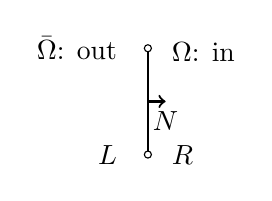
\begin{tikzpicture}[scale=0.45]
    \draw[thick] (0.0,0.0) -- (0,-3) ;
    \draw[->,thick] (0,-1.5) -- (0.5,-1.5) node [below] {$\vect{N}$};
    %\draw[->] (0,-1.5) -- (1,-1.5) node [below] {$\xi$};
    \node[left] at (-0.6,-3) {$L$};
    \node[right] at (.4,-3) {$R$};
    \node[left] at (-0.6,0) {$\bar{\Omega}$: out};
    \node[right] at (.4,-0.1) {$\Omega$: in};
    \draw [fill=white] (0,0) circle (0.1);
    \draw [fill=white] (0,-3) circle (0.1);
  \end{tikzpicture}	
\end{scriptsize}

%%% Local Variables:
%%% mode: latex
%%% TeX-master: "../../presentation"
%%% End: